\subsection{Generate Virtual Content}

Creating virtual content has been at the foundations of computer graphics since its inception. Many processes have been developed over the years to solve the problem. Our aim was to create a digital character (dragon) which could fly around the real environment. Due mostly to our background in the movie industry, we have chosen a workflow designed for digital artists and facilitated by commercial software, namely Autodesk Maya. The process consists of the following steps:

\begin{enumerate}
	\item Modeling 
	\item Texturing or Look-Development
	\item Rigging or Character Setup
	\item Animating
\end{enumerate}

Each of these steps consists of an additive process where elements are added upon the output of the previous step and are pushed further down the chain. Typical workflows are designed such that for as many steps as possible, modifications will be non-destructive to steps further down the chain.

Modeling can be likened to digital sculpture; the primary goal being the creation of a mesh, usually polygonal, that represents the object being created. The two dimensional polygons represent the outer surface of the object or character and are connected in complex patterns to create a three dimensional structure approximating the surface of the object. The exact layout of the polygons does not matter for the look of the object, however considerations must be made for the steps further down the pipeline. Texturing becomes more difficult if large polygons are connected to small polygons, so even distribution is sought after, while rigging becomes more difficult if the edges of the polygonal faces do not align with the axis of movement, so typically quadrilateral polygons are chosen. The output of modeling is a mesh.

Texturing and look-development can be likened to painting a sculpture; it is primarily concerned with the look of the surface that was created by modeling. This is achieved through various means of defining the color generated by the mesh when it is rendered. This can be achieved both by manipulating the texture of the object and by changing the shader it is rendered with. Textures are similar to wallpaper or gift wrap: it spreads a flat image across the surface of a polygon shape either by use of UVs\cite{catmull1974subdivision} or a more complex process such as Ptex. Shading defines how the surface is shown when rendered and typically involves manipulating light from multiple sources to create a color. The output of texturing and look-development is a textured and shaded mesh. 

Rigging or character setup is like taking a sculpture or statue and turning it into a puppet; it is the process of adding the capability of motion to the mesh. While many different means of creating motion exist, the simplest involves three steps: adding bones or joints, adding controls to manipulate the joints, and binding the joints to the mesh with a deformer. Joints consists of hierarchical transforms which can easily be transformed to create complex motion. They can be likened to the bones inside any animal. Controls are the means by which the animator will move the joints in complex ways. Accommodating the needs of the animator should be of utmost consideration - simple controls that are intuitive but give complete control are the goal. To this end tools such as inverse kinematics (IK), forward kinematics (FK), and space switching are employed. In order to let the joints drive the mesh, a deformer, which encodes a complex series of mappings from joints to vertices on the mesh, is used. The process of creating and altering the mappings is called skinning and the key consideration is creating natural looking motions which are both smooth and volume preserving. The output of rigging is a character rig.

Animating is the process of creating motion over time. The character rig is posed using the controls that were set up and keys are set on a particular frame such that the attributes which are keyed will evaluate to the set value when given the frame. Just as in any continuous function, the values between keys are interpolated. The method of interpolation can be controlled so that the desired motion is achieved. The output of animation is a mesh moving through time.

\subsubsection{A Dragon Comes to Life}
In following the traditional animation pipeline, we determined that we did not have enough time and it was outside of our scope to create an entire character from scratch, so we sought out a character model online. Of all the dragons which can be obtained for free online, only one was created with rigging in mind. It was modeled using quads and textured and even provided a rig\cite{dragon}. We proceeded to animate the dragon in a flying sequence such that it would be able to fly around the real room environment around the user.
\begin{figure}[ht]
	\centering
	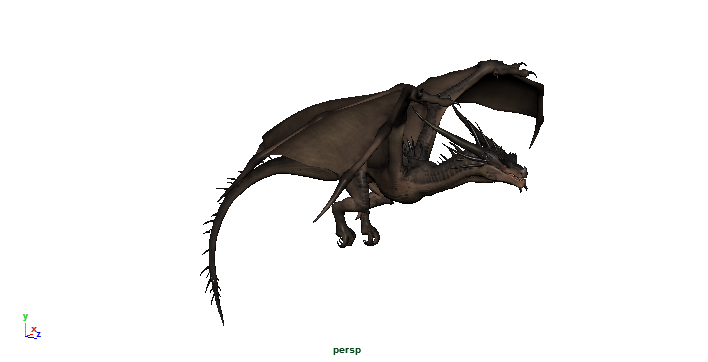
\includegraphics[width=3.0in]{images/cycle.0012.png}
	\caption{A sample frame of our dragon flight animation.}
	\label{fig:dragon}
\end{figure}
As we did not use a game engine for our application, we did not have a freely built-in deformer that could manipulate our dragon mesh over time. It was also outside the scope of this project to create a deformer, so we needed a solution. Our solution was to export our animation sequence frame by frame into the .obj format, which contains both polygonal and texture data. We then would load all the frames into memory and render them in sequence. Thus it was that a dragon came to life.
